\chapter{绪论}\label{chap:introduction}

\section{电缆通道检测机器人的研究背景与意义}
随着城市基础设施建设和电力系统规模的不断扩大，高压电缆通道的数量和分布范围呈现快速增长趋势。电缆通道作为电力输配系统的重要组成部分，承担着电能输送和设备保护的关键任务，其运行状态直接关系到电力系统的安全与稳定。然而，传统的人工巡检与验收方式存在以下几个突出问题：

1）效率低。人工进入电缆通道进行验收，不仅需要耗费大量人力物力，而且在长距离、多分支的电缆沟环境中，检测周期长、效率难以保障；

2）风险高。电缆通道通常位于有限空间或地下环境，通风、照明条件不足，甚至存在有害气体积聚、积水、塌方等潜在危险，人工作业存在较高安全风险；

3）精度不足。人工验收方式主要依靠经验判断，难以对电缆沟内部的几何尺寸、构筑物状态、环境参数等进行高精度、全覆盖的数据采集，容易出现漏检和误判。
在电力行业对智能化、无人化运维要求日益提升的背景下，研发 电缆通道检测机器人已成为解决上述问题的有效途径。该类机器人能够在狭窄、复杂的电缆沟环境中自主运动，搭载多传感器实现 结构尺寸测量、环境参数监测、缺陷识别与三维建模等任务，从而显著提升验收工作的效率、安全性与精度。

\section{电缆通道检测机器人方案选择}
本毕设拟围绕电缆通道检测机器人底盘运动控制与路径规划问题展开研究，重点针对复杂环境下的轮腿式底盘运动控制器设计与基于深度强化学习路径规划算法仿真优化进行探索。通过建立机器人动力学与运动学模型，并结合强化学习策略实现路径规划，以期为电缆通道自动化验收提供可靠的技术支撑。
    
在众多移动机器人底盘方案中，常见的结构包括轮式、足式以及轮腿式。其中，轮式机器人结构简单、运动效率高，但在复杂电缆沟环境下面对障碍物、台阶或坑洼路面时通过性不足；足式机器人机动性强，越障能力突出，但其驱动机构复杂、能耗高、运动控制难度大，不利于在狭长电缆沟中长时间作业。

相比之下，轮腿式机器人结合了轮式与足式的优势：在平整路段可依靠轮式运动实现高效行驶，在遇到障碍物、台阶、井口等复杂地形时可通过足式运动辅助越障，兼顾了高效性与环境适应性。特别是并联式五连杆等新型轮腿机构，能够在保持结构紧凑的同时提供较高的支撑刚度与灵活的运动模式，非常契合电缆通道狭窄空间、复杂地形的应用场景。

机器人在电缆沟中行进的过程中，往往并不具备完整、精确的全局地图信息，仅能通过传感器获取有限的局部环境感知结果，并依据大致的行进方向逐步前进。这种情况下，机器人需要具备实时的路径规划能力，以便在面对障碍物、狭窄通道或环境动态变化时，能够快速决策并调整运动轨迹，从而保障任务的连续性与安全性。

在传统的路径规划方法中，动态窗口法（Dynamic Window Approach，DWA） 被广泛应用。该方法通过搜索机器人速度空间中的候选速度对，结合障碍物距离、速度约束与目标方向等代价函数，选取最优运动指令。虽然 DWA 算法结构清晰、实时性强，但它对环境建模依赖较大，在复杂或动态障碍环境下容易出现局部最优问题（如陷入局部死胡同），且需要人工设计代价函数，鲁棒性和泛化性不足。

相比之下，深度强化学习（Deep Reinforcement Learning，DRL） 为路径规划提供了新的解决思路。通过与环境的交互，DRL 能够在无须显式建模和人工设计代价函数的情况下，直接学习感知状态到控制动作的映射关系，有着自适应能力强，便于处理动态环境，多次交互中学习到更符合任务目标的全局最优行为，而不局限于局部贪婪优化等优势。

\section{电缆通道检测机器人国内外研究现状}

\subsection{底盘结构方案：轮腿式底盘机器人}
2017年，Boston Dynamics公司曝光了一款轮式机器人Handle演示的视频[12]，其最大特点是集轮子和腿为一体，兼具了轮式机器人和腿式机器人的优势。该机器人高约1.98m，重82kg，行进速度约14km/h，垂直跳跃高度约1.2m，一次充电的续航能力约为24km，可搬运45kg以上的重物，还能在多种恶劣环境下顺利行动，如山地,雪地和崎岖的地形。

\begin{figure}[H]
  \centering
  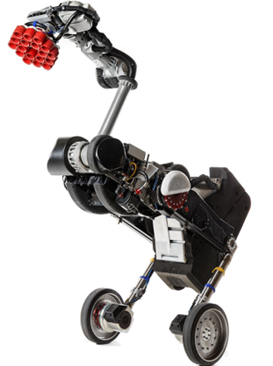
\includegraphics[width=0.5\textwidth]{figures/boston_handle.png}
  \caption{Boston Dynamics公司的轮腿式机器人Handle}
  \label{fig:boston-dynamics-handle}
\end{figure}

苏黎世联邦理工（ETH Zurich）的学生团队Victor Klemm 等人于2018 年9 月研制出了名为Ascento 的双轮跳跃机器人，[13]该机器人主要用于室内巡检，平整地面用轮子快速移动，并通过跳跃来越障。机械结构方面Ascento腿部采用四连杆机构，使整车结构紧凑。Ascento 通过线性二次调节器 (LQR)实现机器人的平衡和运动控制。对于跳跃和坠落恢复的机动过程，则使用带有反馈跟踪的顺序前馈控制器。跌倒恢复的控制策略是该机器人的一大创新，总结了轮腿式双足机器人跌倒后可能会出现的四种稳定位姿，并提出收缩腿部、受控伸展、施加力矩三个恢复步骤。

\begin{figure}[H]
  \centering
  
\includegraphics[width=0.4\textwidth]{eth_1.png}
  \hspace{1cm}
  
\includegraphics[width=0.4\textwidth]{eth_2.png}
  \caption{Ascento机器人实物图（左）与简化图示（右）}
  \label{fig:eth-ascento}
\end{figure}


腾讯 AI Lab 及 Robotics X 实验室主任张正友博士在机器人行业顶会 ICRA 2021 做大会报告，分享了研发中的轮腿式机器人Ollie [14]，在视频中表现了双轮平衡、多模态移动、跳跃、360度空翻等运动能力。Ollie单腿采用并联机构，与身体形成五连杆结构，使整体具有结构简单、动态性能高、爆发力强的特点。机器人基本运动控制采用LQR控制器，此外为适应更多复杂场景，补充采用了IDA-PBC（interconnection and damping assignment- passivity-based control）。

\begin{figure}[H]
  \centering
  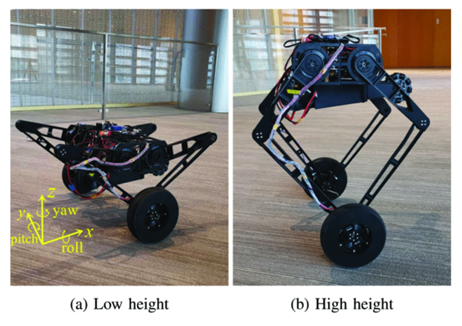
\includegraphics[width=0.5\textwidth]{figures/ollie.png}
  \caption{腾讯AI实验室研发的轮腿式机器人Ollie}
  \label{fig:tencent-ollie}
\end{figure}

\subsection{路径规划算法方案：基于深度强化学习的路径规划算法}

Tai et al.[15]提出了一种基于CNN的DRL模型，该模型以原始RGB-D图像为输入，移动机器人的控制命令为输出。CNN网络的初始权值来自于他们之前工作[13]中训练的参数。但是，由于奖励函数的设计没有涉及鼓励探索的机制，因此该模型只能在简单的走廊环境中实现避障。Jiang等人[17]提出了一种基于启发式制导和避障知识的DQN算法，在路径规划的训练效率和环境适应性方面取得了一定的效果。然而，由于启发式知识限制了DRL智能体的探索能力，规划的路径在路径长度和平滑度方面并不令人满意。[18] Niroui等人研究了一种将DRL与传统的基于边界的方法相结合的勘探模型。DRL模型输出边界点的权重参数，然后根据预定义的代价函数计算出代价最低的边界点。Chen等人[19]提出了一种基于DRL的探索方法，该方法以局部网格图为状态空间，动作空间为随机集合。Zhu等人[20]提出了一种分层DRL网络框架，其中低层DRL策略使机器人在向目标位置移动的同时与障碍物保持安全距离，高层DRL策略作为补充，进一步提高路径规划的安全性。同时，通过选择子目标节点减少状态空间，避免稀疏奖励，该方法在采样效率和迁移能力上都取得了出色的表现。

\paragraph{子段落标题}

子段落标题是最细粒度的标题层级，编号采用小写字母（a、b、c）。在实际论文写作中，通常不建议使用超过三级的标题层级，以保持文章结构的清晰性。

\section{列表}

列表是论文中常用的排版元素，本节展示无序列表和有序列表的使用方法。有序列表的编号格式已按照同济大学毕业设计（论文）撰写规范进行配置。

\subsection{无序列表}

无序列表适用于列举不需要特定顺序的内容，使用 \texttt{itemize} 环境实现。

\begin{itemize}
    \item 同济大学概述：同济大学是一所以工科著称的综合性大学，具有深厚的历史和优秀的教学资源，是中国著名的高等学府之一，享有盛誉。
    \begin{itemize}
        \item 创建于1907年：同济大学始建于1907年，是中国历史最悠久的大学之一，拥有悠久的历史和丰富的文化底蕴；
        \item 位于上海市：校园位于中国上海市，这里是中国经济和文化的重要中心，为学生提供了广阔的发展空间，是学习和生活的理想之地，也是中国高等教育的重要基地；
        \item 以工科著称：同济大学在工程学科方面享有盛誉，是中国顶尖的工科学府之一，培养了大批优秀的工程技术人才，为国家的工程建设和科技创新做出了重要贡献。
    \end{itemize}
    \item 校园文化：同济大学注重校园文化建设，营造了丰富多彩的校园生活。这里的文化活动多样，包括学生社团、艺术节、体育赛事等，为学生提供了展示才华和发展兴趣的平台。
    \item 学术成就：同济大学在多个领域取得了显著的学术成就，培养了大批优秀人才。学校在科学研究、技术创新和社会服务方面都有突出的表现，为国家和社会的发展做出了重要贡献。
\end{itemize}

\subsection{有序列表}

有序列表适用于列举需要按顺序排列的内容，使用 \texttt{enumerate} 环境实现。

需要注意的是，根据同济大学提供的理工科毕业设计（论文）撰写规范，有序列表的第一级编号应使用全角圆括号内的数字，如“（1）”、“（2）”等；第二级编号应使用圆圈内的阿拉伯数字，如“\Circled{1}”、“\Circled{2}”等。此外，有序列表的第二级应为行内列表，即不应另起一行，而应与上一级列表项在同一行内；我们在写 \LaTeX{} 代码时，应该使用 \texttt{enumerate*} 环境来实现有序列表的第二级。

\begin{enumerate}
    \item 同济大学历史：同济大学是中国著名的高等学府之一，拥有悠久的历史和丰富的文化底蕴。以下是同济大学的重要历史节点：
    \begin{enumerate*}
        \item 1907年：创建，最初为德文医学堂；
        \item 1927年：成为国立大学，更名为同济大学；
        \item 1952年：调整学科设置，成为以工科为主的综合性大学。
    \end{enumerate*}
    \item 学术体系：同济大学在学术方面具有很高的声誉，涵盖多个重要学科领域。主要学科包括：
    \begin{enumerate*}
        \item 工程学，包括土木工程、建筑工程、机械工程等；
        \item 建筑学，包括建筑设计、城市规划等；
        \item 医学，包括临床医学、药学等。
    \end{enumerate*}
    \item 国际合作：同济大学积极参与国际交流与合作，拓展全球视野，提升国际影响力。主要的合作项目包括：
    \begin{enumerate*}
        \item 德国交流项目，包括学生交换、教师访问等；
        \item 全球合作伙伴，包括国际知名大学、科研机构等；
        \item 国际学术会议，包括学术研讨会、国际学术交流等。
    \end{enumerate*}
\end{enumerate}

\section{字体}

本模板正文默认使用宋体，标题使用黑体。以下展示模板中可用的中文字体及其效果：

\begin{itemize}
    \item {\songti 宋体}：使用命令 \texttt{\textbackslash songti}。
    \item {\heiti 黑体}：使用命令 \texttt{\textbackslash heiti}。
    \item {\fangsong 仿宋}：使用命令 \texttt{\textbackslash fangsong}。
    \item {\kaishu 楷书}：使用命令 \texttt{\textbackslash kaishu}。
\end{itemize}

\subsection{字号设置}

本模板已按照同济大学毕业设计（论文）撰写规范预设了各部分的字号，一般无需手动调整。如有特殊需要，可使用 \verb|\zihao{}| 命令设置字号，例如 \verb|\zihao{-4}| 表示小四号。常用字号对应关系如\tabref{tab:font-sizes}所示。

\begin{table}[htbp]
  \centering
  \caption{常用字号对照}\label{tab:font-sizes}
  \begin{tabular}{ccl}
    \toprule
    \textbf{字号命令} & \textbf{字号名称} & \textbf{用途} \\
    \midrule
    \texttt{\textbackslash zihao\{2\}}  & 二号   & 封面课题名称 \\
    \texttt{\textbackslash zihao\{-2\}} & 小二号 & 章标题 \\
    \texttt{\textbackslash zihao\{3\}}  & 三号   & 封面副标题 \\
    \texttt{\textbackslash zihao\{4\}}  & 四号   & 封面信息 \\
    \texttt{\textbackslash zihao\{-4\}} & 小四号 & 正文、节标题 \\
    \texttt{\textbackslash zihao\{5\}}  & 五号   & 脚注 \\
    \texttt{\textbackslash zihao\{-5\}} & 小五号 & 页眉页脚 \\
    \bottomrule
  \end{tabular}
\end{table}

\subsection{文字样式}

常用的文字样式命令包括：\textbf{加粗}（\verb|\textbf{}|）、\textit{斜体}（\verb|\textit{}|）、\underline{下划线}（\verb|\underline{}|）以及\emph{强调}（\verb|\emph{}|）。在中文环境下，\verb|\emph{}| 会自动切换为楷书以示强调。

{\songti

【宋体示例】1900年前后，由埃里希·宝隆创办的“同济医院”正式挂牌。医院的医师大都是“德医公会”成员。他们白天忙于经营自己的诊所，只有傍晚到医院看门诊、动手术。埃里希·宝隆医生看到医院里的医疗力量不足，计划在院内设立一所德文医学堂，招收中国学生，以培养施诊医生。这个计划得到德国驻沪总领事以及德国政府高等教育司的支持。1906年，他们设立了一个支持医学堂开办的基金会，得到了德国“促进德国与外国思想交流的科佩尔基金会”的协助，筹集到一批医科书刊及新式的外科手术电动器械等物品。}

{\heiti 【黑体示例】1907年6月医学堂开学前，德国驻沪总领事克纳佩在上海不仅号召德国商人捐款，而且要求德国洋行向中国商人募捐。同时，费舍尔还要求中国官方的资助和支持，克纳佩利用在中德两国募来的捐款，成立了“为中国人办的德国医学堂基金会”。当时规定，捐款金额较多者可成为医学堂董事会董事。医学堂建立时定名为德文医学堂，并成立了董事会负责学校的管理。董事会由18人组成，主要成员有：三个德医公会元老：宝隆、福沙伯（第二任校长）、福尔克尔；三名德国商人：莱姆克、米歇劳和赖纳；两名中国绅商：朱葆三（沪军都督府财政部长及上海商务会会长，大买办）、虞洽卿（荷兰银行买办）；总领事馆的副领事弗赖海尔·冯·吕特等。埃里希·宝隆医生被正式推选为董事会总监督（董事长）兼学堂首任总理（校长），负责学堂的管理。医学堂的校址设在同济医院对面的白克路（今凤阳路415号上海长征医院内）。1907年10月1日德文医学堂举行了开学典礼。}

{\ifcsname fangsong\endcsname\fangsong【仿宋示例】\else[无 \cs{fangsong} 字体。]\fi
1923年3月17日北洋政府教育部下达第108号训令，批准同济工科“改为大学”。学校随即召开董事会议，将学校定名为“同济大学”。1923年3月26日，学校以“同济大学董事会”名义呈文北洋政府教育部，称“经校董会议定名称为同济大学”。1923年4月24日，北洋政府教育部下达第634号“指令”，称“该校名称拟改为同济大学，应予照准备案”。1924年5月20日北洋政府教育部下达第120号训令，批准同济医科为大学。从此以后，5月20日定为校庆日。}

{\ifcsname kaishu\endcsname\kaishu【楷书示例】\else[无 \cs{kaishu} 字体。]\fi
抗日战争胜利后，1946年，国立同济大学分批迁回上海。由于缺少校舍，学校分散教学，成为斜跨上海市区、分散十多处的“大学校”。其中学校办公室和医学院位于善钟路100弄10号（今常熟路），附属医院分别为白克路上的中美医院（原宝隆医院，今凤阳路）和同孚路82号（今石门一路）的原德国医院，理学院在平昌街日本第七国民学校内（今国顺路上海电视大学），文法学院在四川北路（今复兴初级中学），新生院位于江湾新市区的市图书馆（今黑山路），高级工业职业学校则在江湾魏德迈路（今邯郸路），附属中学位于市博物馆（今长海医院飞机楼）。工学院位于其美路的原日本中学（今杨浦区四平路1239号），1949年后逐步发展成同济大学的主校区。}

